\documentclass{article}

\usepackage{fancyhdr}
\usepackage{extramarks}
\usepackage{amsmath}
\usepackage{amsthm}
\usepackage{amsfonts}
\usepackage{tikz}
\usepackage[plain]{algorithm}
\usepackage{algpseudocode}
\usepackage{graphicx}
\usepackage{mcode}
\usetikzlibrary{automata,positioning}

%
% Basic Document Settings
%

\topmargin=-0.45in
\evensidemargin=0in
\oddsidemargin=0in
\textwidth=6.5in
\textheight=9.0in
\headsep=0.25in

\linespread{1.1}

\pagestyle{fancy}
\lhead{\hmwkAuthorName}
\chead{\hmwkClass\ (\hmwkClassInstructor\ \hmwkClassTime): \hmwkTitle}
\rhead{\firstxmark}
\lfoot{\lastxmark}
\cfoot{\thepage}

\renewcommand\headrulewidth{0.4pt}
\renewcommand\footrulewidth{0.4pt}

\setlength\parindent{0pt}

%
% Create Problem Sections
%

\newcommand{\enterProblemHeader}[1]{
    \nobreak\extramarks{}{Problem \arabic{#1} continued on next page\ldots}\nobreak{}
    \nobreak\extramarks{Problem \arabic{#1} (continued)}{Problem \arabic{#1} continued on next page\ldots}\nobreak{}
}

\newcommand{\exitProblemHeader}[1]{
    \nobreak\extramarks{Problem \arabic{#1} (continued)}{Problem \arabic{#1} continued on next page\ldots}\nobreak{}
    \stepcounter{#1}
    \nobreak\extramarks{Problem \arabic{#1}}{}\nobreak{}
}

\setcounter{secnumdepth}{0}
\newcounter{partCounter}
\newcounter{homeworkProblemCounter}
\setcounter{homeworkProblemCounter}{1}
\nobreak\extramarks{Problem \arabic{homeworkProblemCounter}}{}\nobreak{}

%
% Homework Problem Environment
%
% This environment takes an optional argument. When given, it will adjust the
% problem counter. This is useful for when the problems given for your
% assignment aren't sequential. See the last 3 problems of this template for an
% example.
%
\newenvironment{homeworkProblem}[1][-1]{
    \ifnum#1>0
        \setcounter{homeworkProblemCounter}{#1}
    \fi
    \section{Problem \arabic{homeworkProblemCounter}}
    \setcounter{partCounter}{1}
    \enterProblemHeader{homeworkProblemCounter}
}{
    \exitProblemHeader{homeworkProblemCounter}
}

%
% Homework Details
%   - Title
%   - Due date
%   - Class
%   - Section/Time
%   - Instructor
%   - Author
%

\newcommand{\hmwkTitle}{Homework\ \#4}
\newcommand{\hmwkDueDate}{November 118 2016}
\newcommand{\hmwkClass}{STAT 5444}
\newcommand{\hmwkClassTime}{}
\newcommand{\hmwkClassInstructor}{Professor Scott Leman}
\newcommand{\hmwkAuthorName}{Kevin Malhotra}

%
% Title Page
%

\title{
    \vspace{2in}
    \textmd{\textbf{\hmwkClass:\ \hmwkTitle}}\\
    \normalsize\vspace{0.1in}\small{Due\ on\ \hmwkDueDate }\\
    \vspace{0.1in}\large{\textit{\hmwkClassInstructor\ \hmwkClassTime}}
    \vspace{3in}
}

\author{\textbf{\hmwkAuthorName}}
\date{}

\renewcommand{\part}[1]{\textbf{\large Part \Alph{partCounter}}\stepcounter{partCounter}\\}

%
% Various Helper Commands
%

% Useful for algorithms
\newcommand{\alg}[1]{\textsc{\bfseries \footnotesize #1}}

% For derivatives
\newcommand{\deriv}[1]{\frac{\mathrm{d}}{\mathrm{d}x} (#1)}

% For partial derivatives
\newcommand{\pderiv}[2]{\frac{\partial}{\partial #1} (#2)}

% Integral dx
\newcommand{\dx}{\mathrm{d}x}

% Alias for the Solution section header
\newcommand{\solution}{\textbf{\large Solution}}

% Probability commands: Expectation, Variance, Covariance, Bias
\newcommand{\E}{\mathrm{E}}
\newcommand{\Var}{\mathrm{Var}}
\newcommand{\Cov}{\mathrm{Cov}}
\newcommand{\Bias}{\mathrm{Bias}}

\begin{document}

\maketitle

\pagebreak
\begin{homeworkProblem}
Part 1: \\
\begin{align*}
y_i &= \beta_0 + \beta_1x_i + \epsilon_i (i=1,...,N) \rightarrow \epsilon_i = y_i - \beta_0 - \beta_1x_i
	\rightarrow \epsilon_i = y_i - \beta x_i^T, \beta = [\beta_0, \beta_1]\\
\gamma_i &- Gamma(\frac{1}{2}, \frac{1}{2}) \\ 
\epsilon &- N(0, \sigma^2/\gamma_i) \\
\phi &= 1\sigma^2 \\
P(\beta, \phi, \vec{\gamma}|Y, X) &\propto L(\beta, \phi, \vec{\gamma}|Y, X) * P(\vec{\gamma}) * P(\phi) \\
P(\beta, \phi, \vec{\gamma}|Y, X) &\propto \bigg[ \prod_{i=1}^N \gamma_i^{1/2} \phi^{1/2}
	e^{\frac{-\phi \gamma_i}{2}(y_i - x_i^T \beta)^2}\bigg] * 
	\gamma_i^{\frac{1}{2}-1} e^{\frac{-1}{2}\gamma_i} * \phi^{-1} \\
P(\beta, \phi, \vec{\gamma}|Y, X) &\propto \bigg[ \prod_{i=1}^N \gamma_i^{1/2} \phi^{1/2}
	e^{\frac{-\phi \gamma_i}{2}(y_i - x_i^T \beta)^2}\bigg] * 
	\gamma_i^{\frac{1}{2}-1} e^{\frac{-1}{2}\gamma_i} * \phi^{-1}\\
P(\beta, \phi, \vec{\gamma}|Y, X) &\propto \phi^{N/2} \bigg[ \prod_{i=1}^N \gamma_i^{1/2} 
	e^{\frac{-\phi \gamma_i}{2}(y_i - x_i^T \beta)^2}\bigg] * 
	\gamma_i^{\frac{1}{2}-1} e^{\frac{-1}{2}\gamma_i} * \phi^{-1}\\
\Gamma &= \begin{bmatrix}
    \gamma_1 & 0 & \dots & 0 \\
    0 & \gamma_2 & \ddots & \vdots \\ 
    \vdots & \ddots &\ddots & 0  \\
    0 & \dots & 0 & \gamma_N \\
\end{bmatrix} \\
P(\beta, \phi, \vec{\gamma}|Y, X) &\propto \phi^{N/2} \bigg[ \prod_{i=1}^N \gamma_i^{1/2} \bigg] 
	e^{\frac{-\phi }{2}\sum_{i=1}^N \gamma_i(y_i - x_i^T \beta)^2} * 
	\gamma_i^{\frac{1}{2}-1} e^{\frac{-1}{2}\gamma_i} * \phi^{-1}\\
P(\beta, \phi, \vec{\gamma}|Y, X) &\propto \phi^{N/2} |\Gamma|^{1/2}
	e^{\frac{-\phi }{2} (Y - X^T \beta)^T \Gamma (Y - X^T \beta)} * 
	\gamma_i^{\frac{1}{2}-1} e^{\frac{-1}{2}\gamma_i} * \phi^{-1}\\
P(\beta, \phi, \vec{\gamma}|Y, X) &\propto \phi^{N/2} |\Gamma|^{1/2}
	e^{\frac{-\phi }{2} \big[ Y^T\Gamma Y - 2\beta^T X^T \Gamma Y + \beta^TX^T\Gamma XB \big]} * 
	\gamma_i^{\frac{1}{2}-1} e^{\frac{-1}{2}\gamma_i} * \phi^{-1}\\
P(\beta | -) &\propto e^{\frac{-\phi }{2} \big[ Y^T\Gamma Y - 2\beta^T X^T \Gamma Y + \beta^TX^T\Gamma XB \big]} \\
P(\beta | -) &\propto e^{\frac{-\phi }{2} \big[\beta^TX^T\Gamma XB  - 2\beta^T X^T \Gamma Y \big]} \\
P(\beta | -) & - N(\frac{1}{\phi}(X^T\Gamma X)^{-1} * \phi X^T \Gamma Y,
	\frac{1}{\phi}(X^T\Gamma X)^{-1}) \\
P(\beta | -) & - N((X^T\Gamma X)^{-1} X^T \Gamma Y, \frac{1}{\phi}(X^T\Gamma X)^{-1}) \\
P(\phi | - ) &\propto \phi^{N/2 - 1} 
	e^{\frac{-\phi }{2} \big[ (Y - X^T \beta)^T \Gamma (Y - X^T \beta) \big]} \\
P(\phi | - ) & - Gamma(N/2, \frac{1}{2} * (Y - X^T \beta)^T \Gamma (Y - X^T \beta) )\\
P(\gamma_i | - ) &\propto \bigg[ \gamma_i^{1/2} \bigg] 
	e^{\frac{-\phi }{2} \gamma_i(y_i - x_i^T \beta)^2} * 
	\gamma_i^{\frac{1}{2}-1} e^{\frac{-1}{2}\gamma_i}\\
P(\gamma_i | - ) &\propto \bigg[\gamma_i^{1 - 1} \bigg] 
	e^{\frac{-\phi }{2} \gamma_i(y_i - x_i^T \beta)^2 + \frac{-1}{2}\gamma_i} \\
P(\gamma_i | - ) &- Gamma(1, \frac{\phi}{2}(y_i - x_i^T \beta)^2 + \frac{1}{2}) \\ 
\end{align*} \\
Part 2: \\
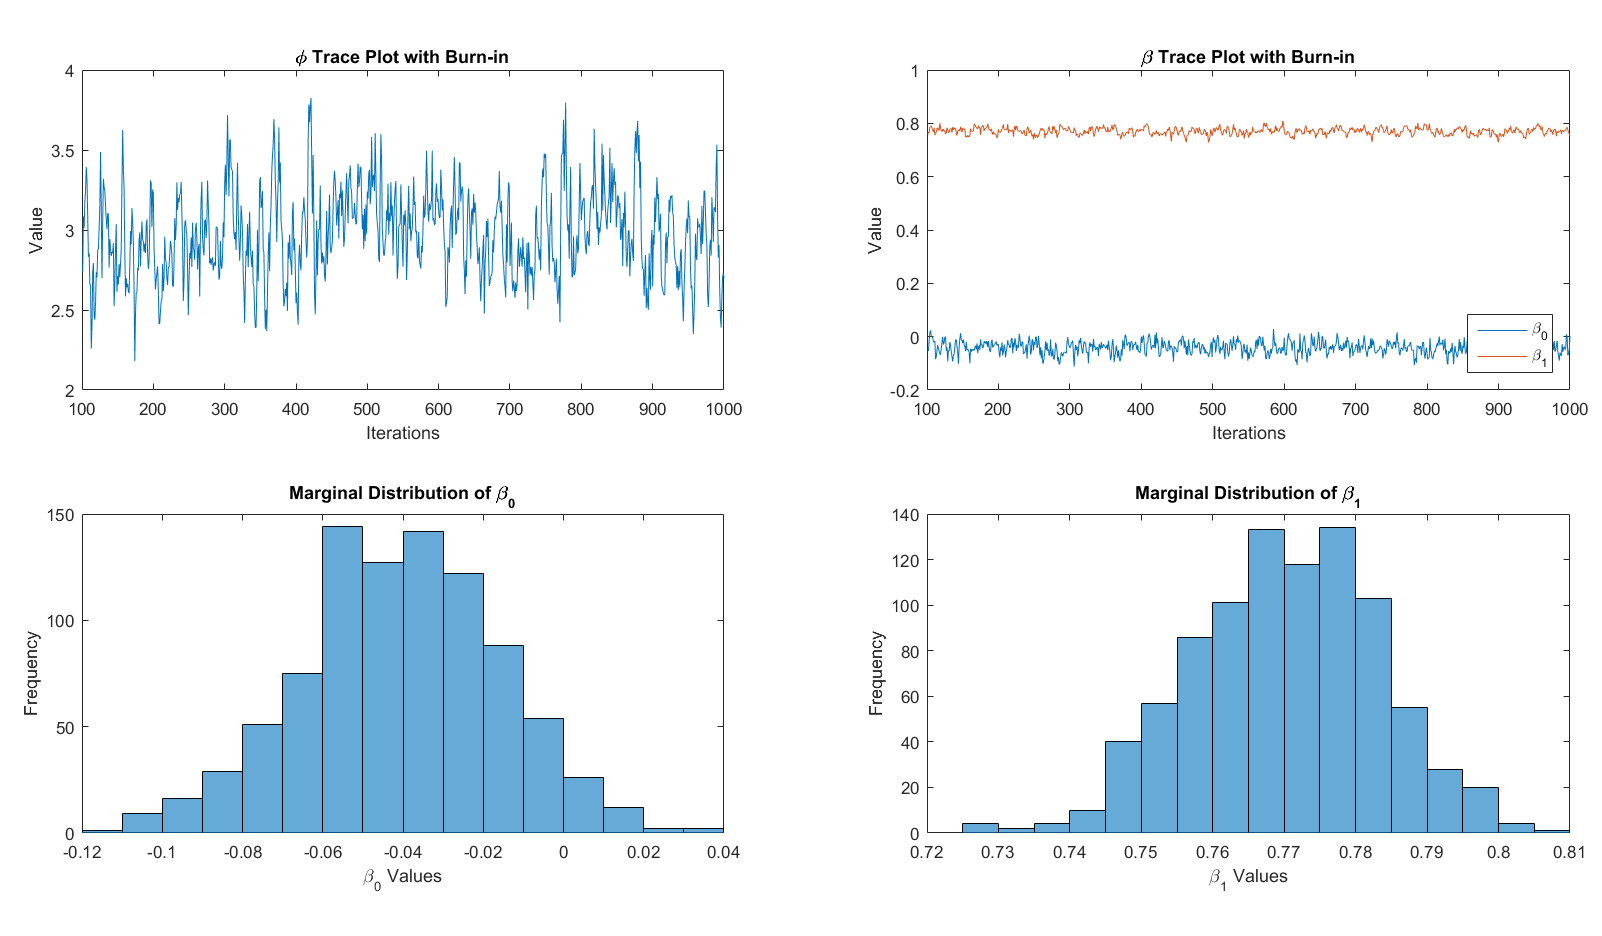
\includegraphics[scale=0.45]{Problem1Part2} \\
\lstinputlisting{HW4_1.m}
\end{homeworkProblem}
\begin{homeworkProblem}
 Part A: \\
 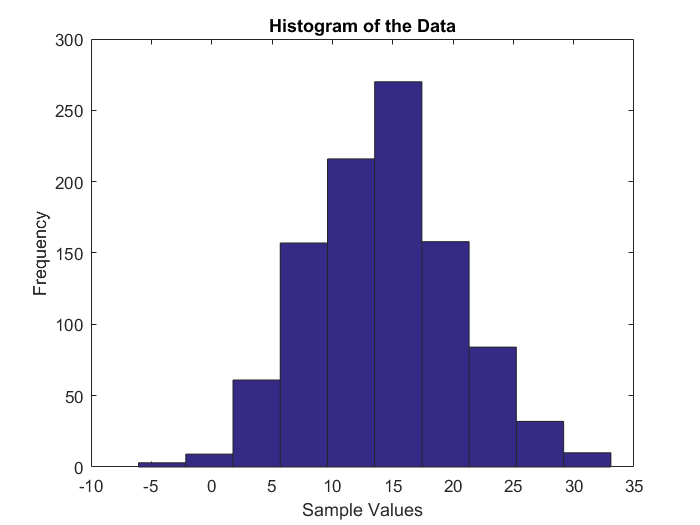
\includegraphics[scale=0.75]{Problem2PartA} \\
 Part B: \\
 \( P(\theta) = \Pi_0 \delta(\theta  = 10) + (1 - \Pi_0)P_{HA}(\theta) \) \\
 \( P_{HA}(\theta)  = \frac{1}{3}\big[ \delta(\theta  = 15) 
 	+ \delta(\theta  = 17) + \delta(\theta  = 20) \big] \) \\
 \( \Pi_0 = \frac{1}{4} \) \\
 Part C: \\
 \begin{align*}
 B &= \frac{\int_{\theta \in H_{0}} L(\theta|X) P_{H_0}(\theta) d\theta}
 	  {\int_{\theta \in H_{A}} L(\theta|X) P_{H_A}(\theta) d\theta} \\
 B &= \frac{\sum_{\theta_i}^{\theta \in H_{0}} L(\theta_i|X)}
 	  {\frac{1}{3}\sum_{\theta_i}^{\theta \in H_{A}} L(\theta_i|X)} \\
H_0 &= \big[ \theta = 10  \big], H_A = \big[ \theta = 15, 17, 20  \big] \\
H_0 &= \big[ \theta = 15  \big], H_A = \big[ \theta = 10, 17, 20  \big] \\
H_0 &= \big[ \theta = 17  \big], H_A = \big[ \theta = 15, 10, 20  \big] \\
H_0 &= \big[ \theta = 20  \big], H_A = \big[ \theta = 15, 17, 10  \big] \\
 \end{align*}
 Part D: \\
 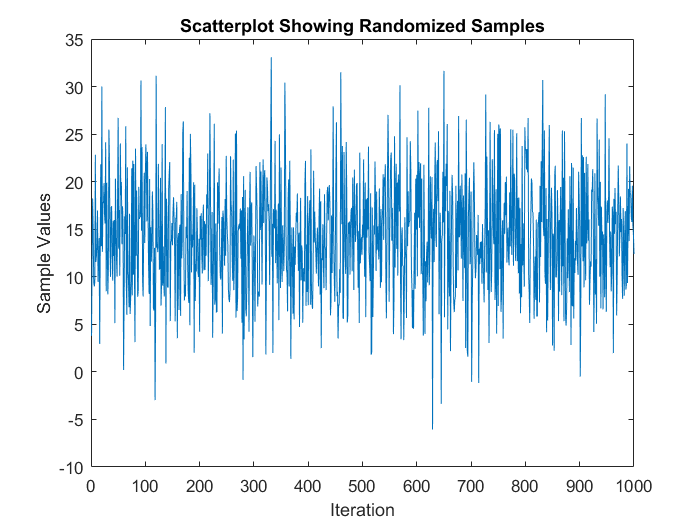
\includegraphics[scale=0.75]{Problem2PartD} \\
 Part E: \\
 \begin{align*}
 P(\theta|X) &\propto L(\theta|X) P_{H_0}(\theta) \\
 P(\theta|X) &\propto \prod_{i=1}^N e^{\frac{-1}{2\sigma^2}(x_i - \mu)^2} \\
 P(\theta|X) &\propto e^{\sum_{i=1}^N\frac{-1}{2\sigma^2}\big[(x_i - \bar{x}) + (\bar{x} - \mu)\big]^2} \\ 
 P(\theta|X) &\propto e^{\sum_{i=1}^N\frac{-1}{2\sigma^2}(\bar{x} - \mu)^2 - 2(x_i - \bar{x})(\bar{x} - \mu)+ (x_i - \bar{x})(x_i - \bar{x})} \\ 
 P(\theta|X) &\propto e^{\sum_{i=1}^N\frac{-1}{2\sigma^2}(\bar{x} - \mu)^2} \\ 
 P(\theta|X) &\propto e^{\frac{-N}{2\sigma^2}(\bar{x} - \mu)^2} \\ 
 \end{align*}
 The following function was used to compute the sequenced posteriors. This is numerically stable algorithm.
 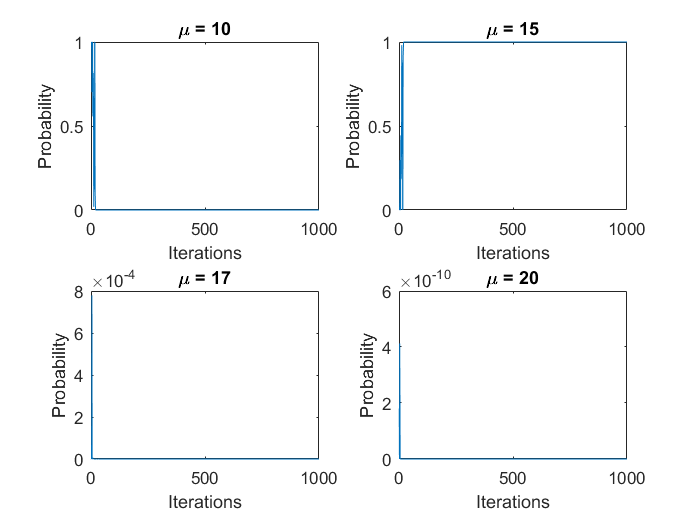
\includegraphics[scale=0.75]{Problem2PartE} \\
 Part E Zoom: \\
 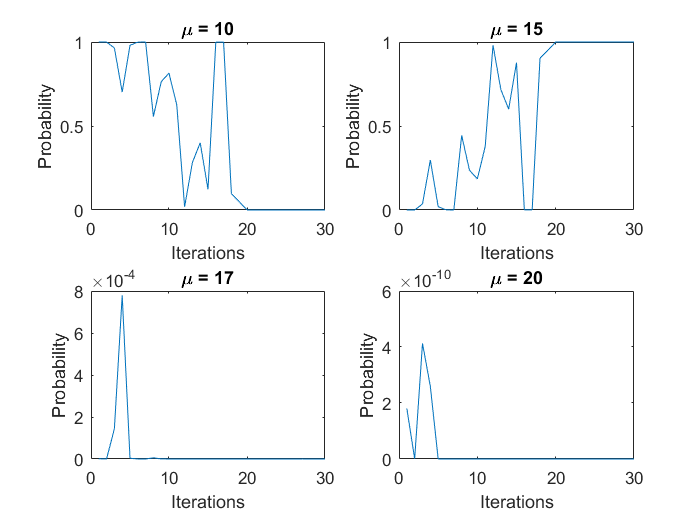
\includegraphics[scale=0.75]{Problem2PartEZoom} \\
 Part F: \\
 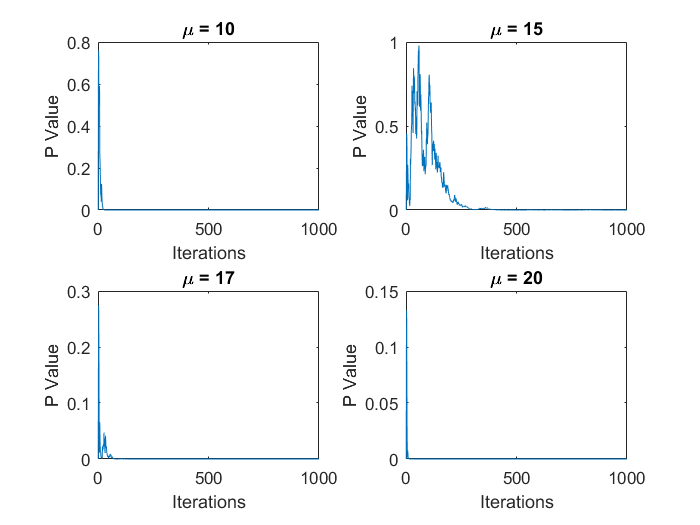
\includegraphics[scale=0.75]{Problem2PartF} \\
 Part F Zoom: \\
 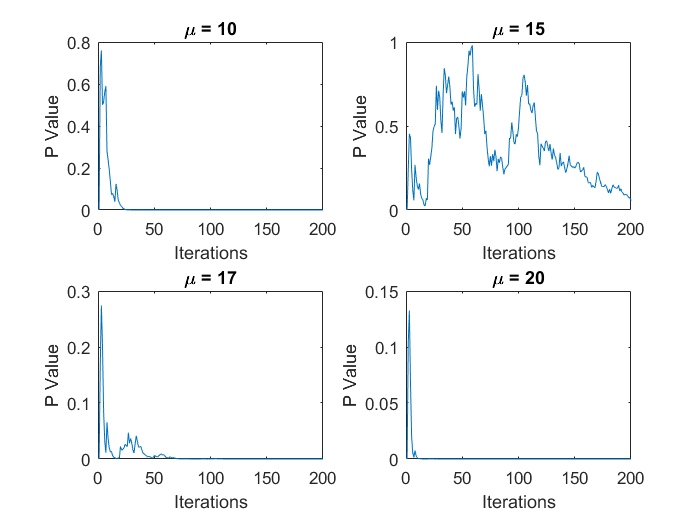
\includegraphics[scale=0.75]{Problem2PartFZoom} \\
 Part H: \\
 We can see that P-Values are not a useful metric for describing the 
 true mean. As we increase sample size the we fail to reject the two tail test for all cases.
 The posterior probabilities kept getting updated with more data points and the mean would
 slowly approach the ground truth mean. The probability would eventually reach 1 for the
 mu that would be closest to ground truth. \\
 Code: \\
 \lstinputlisting{HW4_2.m}
\end{homeworkProblem}
\begin{homeworkProblem}
\begin{align*}
P(H_0|X) &= \frac{\int_{p \in H_0} (X|p) P(p) dP}{\int_{p \in H_0, H_A} P(p) dP} \\
P(X) &=\int_{p \in H_0, H_A} P(X|p) P(p)\\
P(X) &= \int_{p \in H_0, H_A} \bigg[{n \choose k} p^x (1-p)^{n-x}\bigg]
	\bigg[ \gamma(p=0.5)*\frac{1}{1} + p^{\frac{3}{2}-1}(1-p)^{\frac{3}{2}-1} 
	\frac{1}{\beta(\frac{3}{2},\frac{3}{2})} \bigg] *0.5 dp\\
P(X) &= \int_{p \in H_0, H_A} \bigg[{n \choose k} p^x (1-p)^{n-x}\gamma(p=0.5) * 0.5 \bigg] + 
	\bigg[{n \choose k} p^{x+\frac{3}{2}-1}(1-p)^{n-x+\frac{3}{2}-1} 
	\frac{1}{\beta(\frac{3}{2},\frac{3}{2})}  *0.5 \bigg] dp\\
P(X) &= \int_{p \in H_0, H_A} \bigg[{n \choose k} p^x (1-p)^{n-x}\gamma(p=0.5) * 0.5 \bigg] + 
	\bigg[{n \choose k}\frac{ \beta(x+\frac{3}{2}-1, n-x+\frac{3}{2}-1)}
	{\beta(\frac{3}{2},\frac{3}{2})}  *0.5 \bigg] dp\\
P(X) &= \int_{p \in H_0, H_A} \bigg[{n \choose k} p^x (1-p)^{n-x}\gamma(p=0.5) * 0.5 \bigg]dp + 0.5 \\
P(X) &= \bigg[{n \choose k} (p=0.5)^x (1-(p=0.5))^{n-x} * 0.5 \bigg] + 0.5 \\
P(X) &= \bigg[{n \choose k} (0.5)^x (0.5)^{n-x} * 0.5 \bigg]+ 0.5 \\
P(X) &= \bigg[{n \choose k} (0.5)^n * 0.5 \bigg] + 0.5 \\
P(X) &= 0.5 * \bigg[{n \choose k} (0.5)^n + 1 \bigg] \\
P(H_0|X) &= \frac{\int_{p \in H_0} (X|p) P(p) dP}{\int_{p \in H_0, H_A} P(p) dP} \\
P(H_0|X) &= \frac{\int_{p \in H_0} \bigg[{n \choose k} p^x (1-p)^{n-x}\bigg]\bigg[\gamma(p=0.5) * 0.5 \bigg] }{0.5 * \bigg[{n \choose k} (0.5)^n + 1 \bigg]} \\
\end{align*}
\end{homeworkProblem}
\begin{homeworkProblem}
\begin{align*}
p &= P(X \geq t) = 1 - P(X < t) = 1- F(t) = 1- z \\
z &= F(t) \\
\end{align*}
The following information is describing the p-value as a continuous random variable and t an observed measurement. F(X) and F(t) are the cdfs since cdfs are continuous and monotonically increasing we can
write the following.
\begin{align*}
P(X \geq t) &= P(F(X) \geq F(t)) = P(F(X) \geq z) = 1 - z \\
P(X \geq t) &= P(F(X) \geq F(t)) = 1 - P(F(X) < F(t)) = 1 - P(F(X) < z) = 1 - z\\
1 - P(F(X) < z) &= 1 -  z \\
z &= P(F(X) < z) \\
\end{align*}
This states that no matter what sample t we choose the probability that F(t) is less than the continuous random variable cdf will always be the same. This value is the F(t). Thus, in the null hypothesis the P-Value has a uniform distribution since all F(t) values will be same probability regardless of preexisting distribution or the t value. This is the goal of the p-value in the null space.  
\end{homeworkProblem}
\end{document}
